\documentclass[12pt]{article}
% Эта строка — комментарий, она не будет показана в выходном файле
\usepackage{ucs}
\usepackage[utf8x]{inputenc} % Включаем поддержку UTF8
\usepackage[russian]{babel}  % Включаем пакет для поддержки русского языка
\usepackage{amsmath}
\usepackage{amssymb}
\usepackage{mathtools}

\hoffset=0mm
\voffset=0mm
\textwidth=170mm        % ширина текста
\oddsidemargin=-0mm   % левое поле 25.4 - 5.4 = 20 мм
\textheight=240mm       % высота текста 297 (A4) - 40
\topmargin=-15.4mm      % верхнее поле (10мм)
\headheight=5mm      % место для колонтитула
\headsep=5mm          % отступ после колонтитула
\footskip=8mm         % отступ до нижнего колонтитула

\title{Лабораторная работа № 2.1:
    Определение $C_p/C_v$ по скорости звука в газе    
}
\date{\today}
\author{Миллер Сергей 494}

\begin{document}
    \maketitle
    \textbf{Цель работы:}1)  измерение частоты колебаний и длины волны при резонансе звуковых колебаний в газе, заполняющем трубу; 2) определение показателя адиабаты по скорости звука с помощью уравнения состояния идеального газа.

    \textbf{Теория.}

    \textbf{Звуковые волны.} 

    В простых гармонических звуковых волнах, распространяющихся вдоль оси $Ox$, изменение давления $\Delta P$ зависит от координаты $x$ и времени $t$ по закону

    \begin{equation}
        \Delta P(x,t) = P_0 cos(\omega t \pm kx).
    \end{equation}

    Два знака в аргументе косинуса соответствуют двум направлени- ям распространения волны. Между круговой частотой $\omega$, волно- вым числом $k$, длиной волны $\lambda$ и скоростью звука $v_\text{зв}$ выполняются соотношения

    \begin{equation}
        v_\text{зв} = \frac{\omega}{k} = \lambda f; \quad k = 2\pi; \quad \omega = 2\pi f;
    \end{equation}
    здесь $f$ — частота волны.
    Важной характеристикой звуковых волн является скорость их
    распространения. Она определяется инерционными и упругими свойствами среды. Скорость распространения продольных волн в безграничной однородной среде определяется выражением:
     
    \begin{equation}
        v_\text{зв} = \sqrt{\frac{dP}{d\rho}}.
    \end{equation}

    Давление $P$ зависит не только от плотности $\rho$, но и от темпе- ратуры $T$ . Поэтому нужно уточнить, в каком смысле понимается производная $\frac{dP}{d\rho}$.
    Колебания плотности и связанные с ними колебания темпера- туры в звуковой волне происходят настолько быстро, а теплопро- водности газов настолько малы, что для таких процессов теплооб- меном можно пренебречь, так что процесс распространения зву- ка можно считать \textit{адиабатическим}. Следовательно, производную $\frac{dP}{d\rho}$ необходимо рассчитывать для адиабатического процесса.


    \textbf{ Первое начало термодинамики.}

    Из закона сохранения энер- гии следует, что тепло $Q$, полученное термодинамической систе- мой, расходуется на изменение её внутренней энергии $\Delta U$ и на совершение работы $A$ над внешними телами:
    \begin{equation}
        Q = \Delta U + A
    \end{equation}
    Для бесконечно малого процесса уравнение (4) принимает вид 
    \begin{equation}
        \delta Q = dU + \delta A
    \end{equation}

    Поскольку внутренняя энергия является функцией состояния системы, для её элементарного приращения использован знак полного дифференциала $dU$ , а приращения и тепла, и работы не являются полными дифференциалами, а $Q$ и $A$ — не функции состояния(
    Для интегрирования должен быть задан весь промежуточный процесс, поскольку результат будет зависеть от его вида, а не только от начального и конечного состояний).

    \textbf{ Работа газа.}

    Рассмотрим расширение газа в цилиндре, закрытом подвижным поршнем. На поршень действует сила $F$ , равная про- изведению давления газа $F$ на площадь поршня $S$. При смещении на малую величину $dx$ газ совершает работу
    \begin{equation}
        \delta A = F dx = P S dx = P dV.
    \end{equation}
    где $dV$  — малое изменение объёма газа.
    Значит полная работа при некотором процессе имеет вид:
    \begin{equation}
        A = \int P(V) dV
    \end{equation}
    А первое начало термодинамики для газов после использования формулы (6) будет иметь вид:
    \begin{equation}
        \delta Q = dU + P dV
    \end{equation}

    \textbf{Теплоемкость}
    Отношение количества тепла $\delta Q$, поглощённого $\nu$ молями газа при некотором процессе, который обозначим ин- дексом $x$, к повышению его температуры на $dT$, делённое на число молей $\nu$, называется \textit{молярной теплоемкостью газа}:

    \begin{equation}
        C = \bigg(\frac{\delta Q}{dT}\bigg)_x / \nu
    \end{equation}

    Будем считать что $U = U(V,T)$ (так как система описывается тремя параметрами: $V,T,P$ но при этом есть уравнение Менделеева-Клапейрона: $P = P(V,T)$).
    Значит полный дифференциал для $U$ имеет следующий вид:

    \begin{equation}
        dU = \bigg(\frac{\delta U}{\delta T}\bigg)_V dT + \bigg(\frac{\delta U}{\delta V}\bigg)_T dV
    \end{equation}

    Подставим его в первое начало термодинамики:

    $  \delta Q = dU + \delta A =  \bigg(\frac{\delta U}{\delta T}\bigg)_V dT + \bigg(\frac{\delta U}{\delta V}\bigg)_T dV + PdV = \bigg(\frac{\delta U}{\delta T}\bigg)_V dT + \bigg[P + \bigg(\frac{\delta U}{\delta V}\bigg)_T \bigg] dV $

    Разделив все на $dT$ найдем теплоемкость $C_x$ в процессе x:

    \begin{equation}
        C_x = C_v + \bigg[P + \bigg(\frac{\delta U}{\delta V}\bigg)_T \bigg] \bigg(\frac{\delta V}{\delta T}\bigg)_x
    \end{equation}

    Здесь производная $\bigg(\frac{\delta V}{\delta T}\bigg)_x$ вычисляется с учётом процесса $x$, при котором происходит подвод тепла, например, при постоянном объёме $(𝑥 = 𝑉 )$, при постоянном давлении $(𝑥 = 𝑃 )$ или другом условии. Величина $C_v = \bigg(\frac{\delta U}{\delta T}\bigg)_V$ в формуле (11) является теп-
лоёмкостью при постоянном объёме(Дейсвительно, это определение совпадает с определением теплоемкости, так как в процессе $V = const$ выполняется $\delta A = 0$ а значит $\detta U = dQ$).

    \textbf{Теплоёмкость идеального газа.}
    В модели идеального газа внут- ренняя энергия определяется только кинетической энергией дви- жения молекул, следовательно, внутренняя энергия идеального газа не зависит от объёма: $\bigg(\frac{\delta U}{\delta V}\bigg)_T = 0$.

    Тогда формула (11) станет более простой:

    \begin{equation}
        C_x = C_v + P \bigg(\frac{\delta V}{\delta T}\bigg)_x
    \end{equation}

    Используя уравнение Менделеева-Клапейрона ($PV = \nu RT$),
    для $C_p$ (то есть процесса $x = P$ с постоянным давлением) получим:

    \begin{equation}
        C_p - C_v = R
    \end{equation}
    где $C_p, C_v$ - \textit{молярные} теплоемкости при постоянных давлении и объеме соответсвенно.

    Отношение этих теплоемкостей называется показателем адиабаты:

    \begin{equation}
        \gamma = \frac{C_p}{C_v}
    \end{equation}

    В нешироком диапазоне температур $C_v$ можно считать постоянной, что соответствует пропорциональности внутренней энер- гии газа его температуре:

    \begin{equation}
        U = \nu \int C_v dT = \nu C_v T
    \end{equation}

    Энергия, переданная молекуле, распределяется между различны- ми формами её движения: поступательным, вращательным и ко- лебательным. В статистической физике доказывается теорема о равномерном распределении энергии между степенями свободы молекулы1, согласно которой на каждую степень свободы прихо- дится в среднем энергия, равная $\frac{RT}{2 N_A}$

    При $i$ степенях свободы, внутренняя энергия $U$ одного моля такого газа и величина $C_v$ равны соответственно

    \begin{equation}
        U = \frac{i}{2}RT; \quad C_v = \frac{iR}{2}; 
    \end{equation}

    где $R = 8,31 \text{Дж}/\text{(моль · К)}$ — универсальная газовая постоянная, $N_A = 6,02 · 1023 \text{моль}^{−1}$ — количество молекул в моле вещества (число Авогадро).
    В рассматриваемом приближении для показателя адиабаты в соответствии с (13) и (14) получим

    \begin{equation}
        \gamma = \frac{i+2}{i}
    \end{equation}

    \textbf{Адиабатический процесс.}

    Квазистатический процесс, проис- ходящий без теплообмена с окружающей средой, называется адиа- батическим.
    Из первого начала термодинамики (6) при $\delta Q = 0$ для $\nu$ молей идеального газа, у которого $dU = \nu C_v dT$, получим:

    \begin{equation}
        \nu C_v dt + P dV = 0,
    \end{equation}

    А так как $PV = \nu RT$, получаем: 

    \begin{equation}
        C_v \frac{dT}{T} + R \frac{dV}{V} = 0
    \end{equation}

    Далее интегрируя и вновь используя уравнение состояния, получим:

    \begin{equation}
        PV^{\gamma} = const
    \end{equation}

    (адиабата Пуассона)

    \textbf{Скорость звука}
    Распространение звуковой волны в газе проис- ходит адиабатически. Сжатия и разрежения в газе сменяют друг друга настолько быстро, что теплообмен между слоями газа, име- ющими разные температуры, не успевает произойти. Используя полученное уравнение адиабаты идеального газа, найдём скорость звука по общей формуле (3).

    Заменим в уравнении Пуассона $PV^{\gamma} = const$ объём на плот- ность $\rho = \frac{m}{V}$ , после чего получим $P = const \rho^{\gamma} $. Тогда после логарифмирования и дифференцирования этого выражения име- ем:

    \begin{equation}
        \frac{dP}{P} = \gamma \frac {d\rho}{\rho}, \quad \text{или} \quad \bigg(\frac{dP}{d\rho}\bigg)_\text{адиаб} = \gamma \frac{P}{\rho},
    \end{equation}

    тогда для скорости звука получаем:

    \begin{equation}
        v_\text{зв}^2 = \bigg(\frac{dP}{d\rho}\bigg)_\text{адиаб} = \gamma \frac{P}{\rho} = \gamma \frac{RT}{\mu},
    \end{equation}
    где $\mu$ - молярная масса газа.

    Преобразуя, получим:

    \begin{equation}
        \gamma = \frac{\mu}{RT}v_\text{зв}^2
    \end{equation}

    Таким образом, для определения показателя адиабаты доста- точно измерить температуру газа и скорость распространения зву- ка (молярная масса газа предполагается известной).

    \textbf{Идея эксперимента}
    Звуковые колебания в трубе являются наложением всех отражённых волн и, вообще говоря, очень сложны. Картина упрощается, если длина трубы $𝐿$ равна целому числу полуволн, то есть когда выполняется условие
    \begin{equation}
        L = n\frac{\lambda}{2}
    \end{equation}
    где $n$ — любое целое число. Совпадающие по фазе волны, бегущие в противо- положных направлениях, складываясь, усиливают друг друга, и образуется стоячая звуковая волна:
    Δ𝑃 (𝑥,𝑡) = 2𝑃0 cos(𝜔𝑡) sin(𝑘𝑥).
    Амплитуда звуковых колебаний при этом резко возрастает — на- ступает резонанс.

    При неизменной частоте 𝑓 звукового генератора (а следова- тельно, и неизменной длине звуковой волны 𝜆) можно из- менять длину трубы 𝐿. Для этого применяется раздвижная труба. Длина раздвижной трубы постепенно увеличивает- ся, и наблюдается ряд последовательных резонансов. Воз- никновение резонанса легко наблюдать на осциллографе по резкому увеличению амплитуды колебаний. Для последова- тельных резонансов имеем

    \begin{equation}
        L_n = n\frac{\lambda}{2}, L_{n+1} = (n+1)\frac{\lambda}{2}, \dots L_{n+k} = n\frac{\lambda}{2} + k\frac{\lambda}{2}
    \end{equation}
    
    т. е. $\lambda/2$ равно угловому коэффициенту графика, изобража- ющего зависимость длины трубы $L$ от номера резонанса $k$. Скорость звука находится по формуле (2).

    \textbf{В работе испольуются:} звуковой генератор (ЗГ); электронный осциллограф (ЭО); микрофон; раздвижная труба; термометр.

    \begin{center} 
    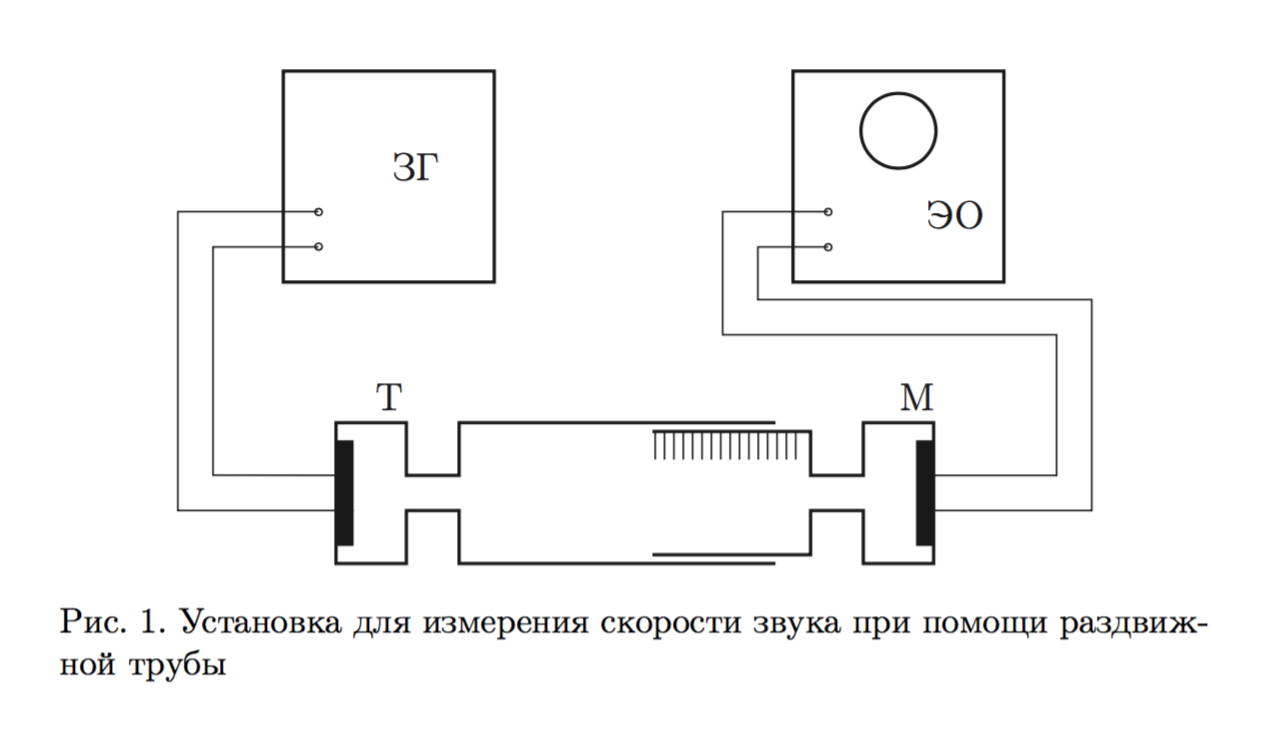
\includegraphics[width=3.5in]{stand.png}
    \end{center}

    \textbf{Ход работы:}

    \begin{enumerate}
    \item 
         Будем медленно удлинять трубу при постоянной частоте и измерять смещение трубы от начального состояния при последовательных резонансах.
    Так как ожидаемая зависимость длины трубы от номера резонанса $f(n)$ линейная, то построим аппроксимирующие по методу наименьших квадратов прямые вида $f = kn + b$ для каждой измеряемой частоты, а также произведем оценку ошибки(для углового коэффицента $k$):

    \begin{equation}
        \hat{k} = \frac{\overline{xy} - \bar{x}\bar{y}}{\overline{x^2} - \bar{x}^2} ;\quad \hat{\sigma}_k = \frac{2}{\sqrt{n}}\sqrt{\frac{\overline{y^2} - \bar{y}^2}{\overline{x^2} - \bar{x}^2} - \hat{k}^2}
    \end{equation}

    Здесь в качестве погрешности для полученной оценки $\hat{k}$  взяли удвоенное стандартное отклонение, в пределах которого в среднем лежит $98\%$ результатов.

    После этого найдем скорость звука: $\hat{v}_\text{зв} = \hat{\lambda} f = 2 \hat{k} f$

    Тогда получим искомое значение показателя адиабаты: $\hat{\gamma} = \frac{4\mu \hat{k}^2 f^2}{RT}$ 

    А погрешность $\hat{\sigma}_\gamma$ определим из формулы для погрешности функции многих переменных:

    \begin{equation}
        \bigg(\frac{\hat{\sigma}_\gamma}{\hat{\gamma}}\bigg) ^ 2 =    2^2 \bigg(\frac{\hat{\sigma}_k}{\hat{k}}\bigg) ^ 2 + 2^2 \bigg(\frac{\hat{\sigma}_f}{\hat{f}}\bigg) ^ 2 + \bigg(\frac{\hat{\sigma}_T}{\hat{T}}\bigg) ^ 2
    \end{equation}

    \begin{itemize}
        \item $f = 1.13$ KГц

        \begin{center}
                    \begin{tabular}{|c|c|c|c|c|c|c|}
                            \hline 
                                $n$ & 1 & 2 & 3 & 4 & 5 \\
                            \hline
                                $f_n$ [мм]& 75&104&130&167&220\\
                            \hline
                    \end{tabular}
        \end{center}

        \begin{equation}
            \hat{k}  ,\quad \hat{\sigma}_k
        \end{equation}

    \end{itemize}

    \end{enumerate}

\end{document}